\documentclass{beamer}
\usepackage{polski}
\usepackage[utf8]{inputenc}

\usetheme{CambridgeUS}
\usecolortheme{seagull}
\setbeameroption{show notes}

\title[Transport dźwigarów w systemie JIT]
{Problem optymalnego transportu dźwigarów w systemie Just in Time}
\author{Izabela Biczysko, Krzysztof Piecuch}
\institute[ii UWr]{Instytut Informatyki Uniwersytetu
Wrocławskiego}
\date{Wrocław, \today}



\begin{document}
 \maketitle

%  **************************************************  Problem optymalnego transportu dźwigarów **********************************************************


\section{Wstęp}
  \begin{frame}
  \frametitle{Agenda}
  \tableofcontents
  \end{frame}


% **************************************************  Problem optymalnego transportu dźwigarów **********************************************************
 
 
 \section{Problem optymalnego transportu dźwigarów}
 \begin{frame}
  \frametitle{Motywacja}
  \begin{itemize}
   \item Firma zajmująca się przebudową sieci transportowej chce zoptymalizować proces transportu dźwigarów na plac budowy
   \item Proces montażu dźwigarów jest ściśle powiązany z innymi pracami budowlanymi
   \item Przekroczenie terminu zamontowania dźwigaru wiąże się z dodatkowymi kosztami
   \item Nie ma możliwości składowanie dźwigarów na placu budowy
   \item Bezpośrednio z dźwigarów pojazdy są umieszczane na podporach
   \item Transport dźwigarów odbywa się w systemie Just in Time (JIT)
  \end{itemize}

 \end{frame}
 
 \begin{frame}
  \frametitle{Zadania}
  Znane są okna czasowe tzn. najwcześniejsze i najpóźniejsze terminy dostawy poszczególnych dźwigarów. 
  Należy znaleźć takie terminy dostawy poszczególnych dźwigarów na plac budowy aby zminimalizować koszty związane z
  przekroczeniem okien czasowych.
  \end{frame}

  \begin{frame}
  \frametitle{{Ograniczenia}}
   \begin{enumerate}
    \item dźwigary należy dostarczyć zgodnie z kolejnością montażu (porządkiem technologicznym)
    \note[item] {dźwigary należy dostarczyć zgodnie z kolejnością montażu (porządkiem technologicznym)  - ten punkt jest bez sensu, zinterpretujmy go tak,
    że mamy okna czasowe i to one wyznaczają kolejność}
    \item jednocześnie pojazd może przewozić tylko jeden dźwigar
    \note[item]{OK}
    \item po załadunku dźwigar może być zdjęty jedynie bezpośrednio przed montażem
    \note[item]{Ewentualnie może być przetrzymywany na pojeździe}
   \end{enumerate}
   \end{frame}
  

%  **************************************************  Transport z najwcześniejszymi i najpóźniejszymi terminami dostawę **********************************************************

\section{Transport z najwcześniejszymi i najpóźniejszymi terminami dostaw}
 \begin{frame}
 \frametitle{Model matematyczny}
 \begin{block}{Zbiór dźwigarów}
  $ \textbf{B} = { B_1, B_2, B_3,...,B_m} $
 \end{block}
 
 \begin{block} {Dla dowolnego dźwigara $ B_i \in \textbf{B} $ wprowadzamy oznaczenia}
 \begin{itemize}
  \item $ z_i $ - czas załadunku
  \item $ t_i $ - czas transportu na plac budowy 
  \item $ r_i $ - czas rozładunku na placu budowy 
  \item $ p_i $ - czas powrotu
  \item $ e_i $ - żądany najwcześniejszy termin przywozu 
  \item $ d_i $ - żądany najpóźniejszy termin przywozu
  \item $ v_i $ - współczynnik funkcji kary za zbyt wczesne przybycie 
  \item $ w_i $ - współczynnik funkcji kary za zbyt późne przybycie
 \end{itemize}
 \end{block}
\end{frame}

 \begin{frame}
 \frametitle{Model matematyczny}
 
 \begin{block}{Założenia}
 Niech:
 \begin{itemize}
  \item kolejność transportu dźwigarów to $(B_1, B_2,...,B_m) $
  \item załadunek pierwszego dźwigara rozpocznie się w chwili 0
  \item $ S_i $ oznacza termin dostarczenia dźwigara $B_i$ na plac budowy 
 \end{itemize}
 \end{block}
\end{frame}

 \begin{frame}
 \frametitle{Model matematyczny}
 
 \begin{block}{Terminy $S_1, S_2,...,S_n $ muszą spełniać następujące ograniczenia}
 \begin{itemize}
    \note[item]{Na ewolucyjne trzeba to wyrzucić i trzeba wymyśleć co zrobimy z ograiczeniami na PO}
    \item załadunek pierwszego dźwigara $B_i$ rozpoczyna się w chwili 0
    \begin{equation}\label{eq:ZeroStart}
     S_1 \ge z_1 + t_1 
    \end{equation}
    \item dźwigary należy dostarczyć zgodnie z kolejnością montażu 
    \note[item]{dźwigary należy dostarczyć zgodnie z kolejnością montażu - bez sensu}
    \begin{equation}\label{eq:Order}
     S_{i+1} \ge S_i , i = 1,2,...,m-1
    \end{equation}    
 \end{itemize}
 \end{block}
\end{frame}


 \begin{frame}
 \frametitle{Model matematyczny}
 
 \begin{block}{Terminy $S_1, S_2,...,S_n $ muszą spełniać następujące ograniczenia}
 \begin{itemize}
       \item jednocześnie pojazd może przewozić tylko jeden dźwigar
     \begin{equation}\label{eq:OneVehicle}
     \begin{split}
      \forall B_i, B_j \in \textbf{B}, S_i - r_i - t_i - z_i \ge S_j - r_j - t_j - z_j
      \\ \   \vee S_j - r_j - t_j - z_j \ge S_i - r_i - t_i - z_i
     \end{split}
     \end{equation}
      \note[item]{jednocześnie pojazd może przewozić tylko jeden dźwigar - nie rozumiem równania}
     \item po załadunku dźwigar może być zdjęty jedynie bezpośrednio przed montażem
      \begin{equation}\label{eq:TakeOff}
      S_{i+1} \ge S_i + r_i + p_i + z_{i+1} + t_{i+1}, i = 1,2,...,m-1
      \end{equation}        
 \end{itemize}
 \end{block}
\end{frame}

\begin{frame}
 \frametitle{Zadanie}
 \begin{block}{}
 Problem transportu dźwigarów sprowadza się więc do wyznaczenia terminów dostaw $S_1, S_2,...,S_n $ spełniających ograniczenia (\ref{eq:ZeroStart})
 - (\ref{eq:TakeOff}), które optymalizują pewne przyjęte kryterium optymalizacyjne
  
 \end{block}
\end{frame}


\begin{frame}
 \frametitle{Transport dokładnie na czas jednym pojazdem}
 \begin{itemize}
  \item dźwigary są transportowane na plac przez dokładnie jeden pojazd
 \end{itemize}
 \begin{block}{}
 \begin{itemize}
 \item $ E_i = max{0, e_i - S_i} $ 
 \item $ T_i = max{0, S_i - d_i} $
 \end{itemize}
 \end{block}
 
 \begin{block}{Kryterium optymalizacyjne}
  \begin{equation}
   F(S) = \sum_{i=1}^{n}(u_iE_i + w_iT_i) 
  \end{equation}
 \end{block}

\end{frame}




% ***************************************************** Pojęcia i twierdzenia *********************************************************************


\section{Pojęcia i twierdzenia}

\begin{frame}

\frametitle{Pojęcia i twierdzenia}
  
 \begin{theorem}\label{th:NoIdle}
  Istnieje optymalne rozwiązanie w którym dla każdego dźwigara i czynności $z_i, t_i, r_i, p_i$ są wykonywane
  pod rząd bez okresów bezczynności
 \end{theorem}
 
 \begin{block}{Uwaga}
  Wobec twierdzenia \ref{th:NoIdle}, niech $j_i = z_i, t_i, r_i, p_i$ będzie praca związaną z dostarczeniem i-tego dźwigara.
 \end{block}

\end{frame}
 



\begin{frame}
\frametitle{Pojęcia i twierdzenia}
  
 \begin{definition}\label{de:block}
  Podciąg $ u, u+1, ... v$ ciągu \textbf{S} = $S_1, S_2,...,S_n $ nazwiemy \alert{blokiem}, jeżeli zadania $j_u, j_{u+1}, j_v $
  są wykonywane pad rząd bez czasu bezczynności, natomiast jest czas bezczynności przed zadaniem u i po zadaniu v.
 \end{definition}
 
 
\end{frame}


% ***************************************************** Algorytm Konstrukcyjny *********************************************************************


\section{Algorytm Konstrukcyjny}

\begin{frame}

\frametitle{Pojęcia i twierdzenia}

\begin{enumerate}
 \item Posortiwać dźwigary zgodnie z najpóźniejszy terminem przywozu
 \item Znaleźć podział na bloki dla zadanej kolejności
 \item Znaleźć optymalny czas dostawy dla każdego dźwigara
\end{enumerate}

\end{frame}



\begin{frame}

\frametitle{Podział na bloki}

\end{frame}


\begin{frame}

\frametitle{Znajdowanie optymalnego czasu}

\end{frame}


% ***************************************************** Wpływ ograniczeń na złożoność czasową *********************************************************************
\section{Wpływ ograniczeń na złożoność czasową}

\begin{frame}
 \frametitle{Wpływ ograniczeń na złożoność czasową}
 ??????????????????
\end{frame}

% *************************************************************Algorytm Ewolucyjny **********************************************************************

\section{Algorytm Ewolucyjny}

\begin{frame}
 \frametitle{Schemat algorytmu}
 \begin{center}
 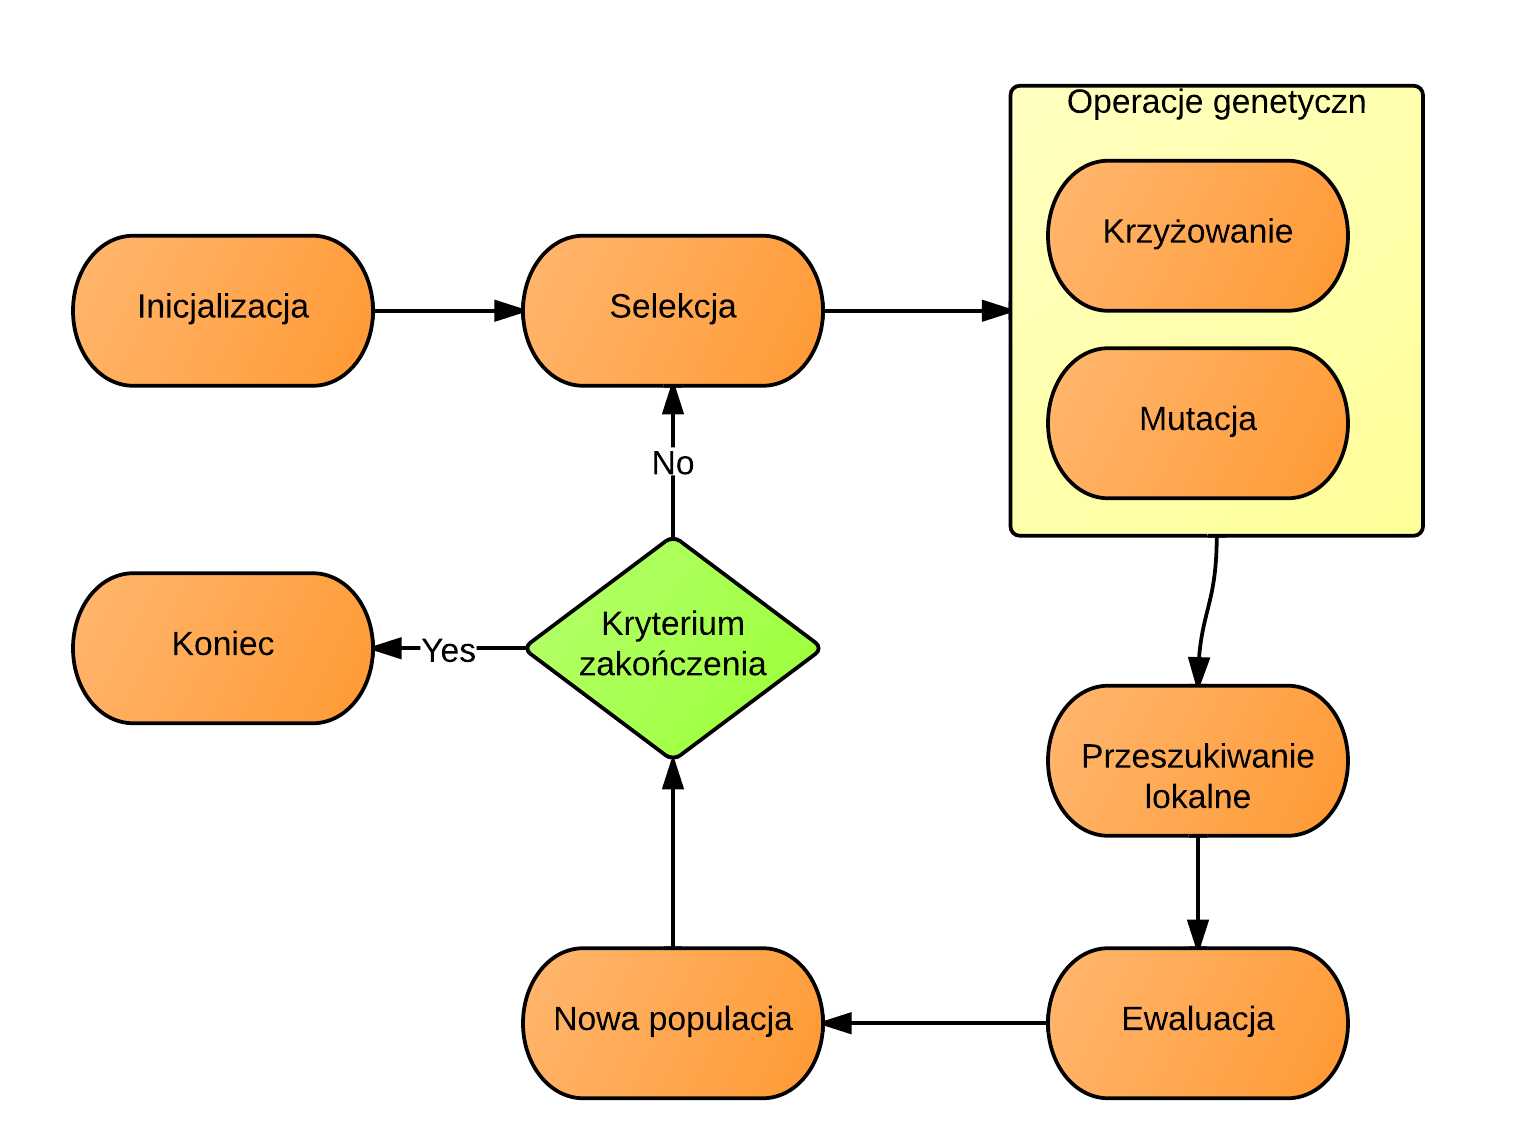
\includegraphics[scale=0.18]{./Grafika/schemat.png}
 % schemat.png: 1517x1123 pixel, 72dpi, 53.52x39.62 cm, bb=0 0 1517 1123
\end{center}

\end{frame}

\begin{frame}
 \frametitle{Inicjalizacja}
 
 

\end{frame}




\end{document}